% arara: xelatex: { synctex: yes, shell: yes, interaction: nonstopmode }
% arara: xelatex: { synctex: yes, shell: yes, interaction: nonstopmode }
% arara: clean: { extensions: [aux, log, toc, out, lof, lot, synctex.gz, fls, fdb_latexmk, xdv] }
\documentclass[11pt,a4paper]{article}

\def\Classe{2nde}
\def\Titre{Probabilité}

\let\nc\newcommand\let\rnc\renewcommand\nc{\m}[1]{\ensuremath{#1}\xspace}\nc{\euro}{€}
\usepackage[french]{babel}
\usepackage{geometry}\geometry{top=2cm, bottom=2cm, left=1.0cm, right=1.0cm}
\usepackage{tikz,pgf}

\usepackage{fancyhdr,lastpage,wrapfig2,enumitem,lipsum}
\setlist[itemize]{label=\textbullet}
\pagestyle{fancy}
\fancyhead{}\fancyfoot{}\rnc{\headrulewidth}{0.4pt}\rnc{\footrulewidth}{0.4pt}
\fancyhead[R]{\normalsize\Classe}\fancyfoot[L]{\normalsize\Titre}\fancyfoot[R]{\normalsize\thepage{}~/~\pageref*{LastPage}}
\makeatletter\fancypagestyle{plain}{\fancyhf{}\rnc{\headrulewidth}{0pt}\rnc{\footrulewidth}{0pt}}\makeatother

\usepackage{fontspec,unicode-math,fontawesome5}
\usepackage{hyperref}\hypersetup{colorlinks=true,linkcolor=blue,urlcolor=blue}

\setmainfont{Lato}
\setmathfont{Latin Modern Math}

\usepackage{xcolor}
\definecolor{mainblue}{RGB}{120,160,220}
\definecolor{softblue}{RGB}{245,248,255}
\definecolor{maingreen}{RGB}{120,180,140}
\definecolor{softgreen}{RGB}{245,252,247}
\definecolor{mainorange}{RGB}{240,180,120}
\definecolor{softorange}{RGB}{255,250,245}
\definecolor{mainred}{RGB}{220,140,140}
\definecolor{softred}{RGB}{255,245,245}

\usepackage{tocloft}\rnc{\cftdotsep}{1}\rnc{\cftsecdotsep}{\cftdotsep}\rnc{\cftsubsecdotsep}{\cftdotsep}\rnc{\cftsubsubsecdotsep}{\cftdotsep}
\usepackage[most]{tcolorbox}
\tcbset{ enhanced, frame hidden, coltitle=black, colback=white, opacityback=0, sharp corners, left=2pt, right=0pt, top=0pt, bottom=0pt }
\newtcolorbox{defi}[1][]{ borderline west={2pt}{0pt}{mainblue}, title={\normalsize\faLightbulb[regular]}~\normalfont\ul{\textbf{Définition :\if\relax\detokenize{#1}\relax\else~#1\fi}} }
\newtcolorbox{theo}[1][]{ borderline west={2pt}{0pt}{mainred}, title={\normalsize\faThumbtack}~\ul{\textbf{Théorème :\if\relax\detokenize{#1}\relax\else~#1\fi}} }
\newtcolorbox{prop}[1][]{ borderline west={2pt}{0pt}{maingreen}, title={\normalsize\faCheck}~\ul{\textbf{Propriété :\if\relax\detokenize{#1}\relax\else~#1\fi}} }
\newtcolorbox{ex}[1][]{ left=-5pt, title=\ul{\textbf{Exemple :\if\relax\detokenize{#1}\relax\else~#1\fi}} }
\newtcolorbox{rem}[1][]{ left=-5pt, title=\ul{\textbf{Remarque :\if\relax\detokenize{#1}\relax\else~#1\fi}} }
\newtcolorbox{void}{ left=-5pt }

\usepackage{ulem,contour}\rnc{\ULdepth}{1.5pt}\rnc{\ULthickness}{0.5pt}\contourlength{0.8pt}\nc{\ul}[1]{\uline{\phantom{#1}}\llap{\contour{white}{#1}}}
\usepackage{titling}\setlength{\droptitle}{-2cm}
\title{}\author{}\date{}
\pretitle{\begin{center}\begin{tikzpicture}\def\rectwidth{\textwidth}\def\rectheight{4cm}\begin{scope}\clip(0,0)rectangle(\rectwidth,\rectheight);\IfFileExists{img/image.png}{\node[anchor=center,opacity=0.2]at(\rectwidth/2,\rectheight/2){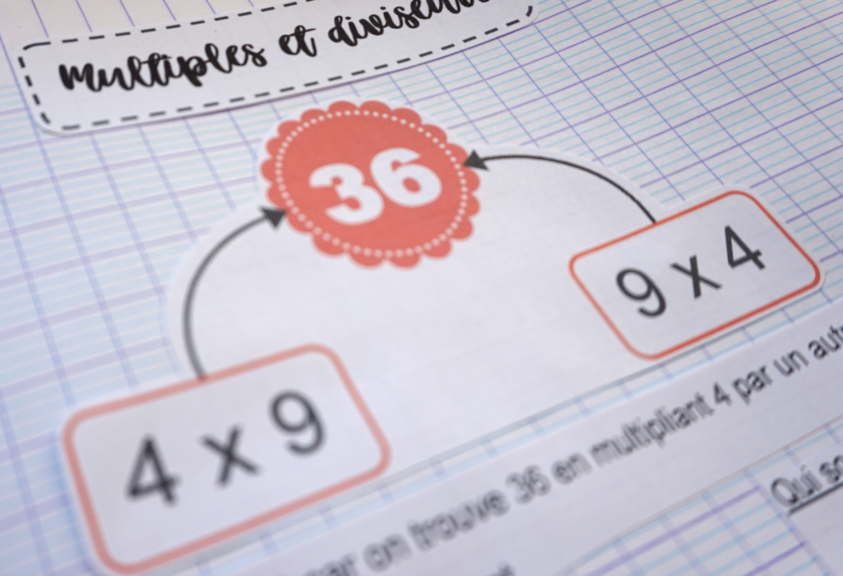
\includegraphics[width=\textwidth]{img/image.png}};}{}\end{scope}\node[align=center]at(\rectwidth/2,\rectheight/2){\Huge\bfseries\Titre};\end{tikzpicture}\end{center}}
\posttitle{}

\usepackage{titlesec}\titleformat{\section}{\normalfont\Large\bfseries}{\thesection.}{0.5em}{\ul}\titleformat{\subsection}{\normalfont\large\bfseries}{\thesubsection.}{0.5em}{\ul}\titleformat{\subsubsection}{\normalfont\normalsize\bfseries}{\thesubsubsection.}{0.5em}{\ul}

\nc{\prob}{\mathbb{P}}
\nc{\esp}{\mathbb{E}}
\nc{\var}{\mathrm{Var}}

\begin{document}
\maketitle
\vspace{-3cm}
\tableofcontents

\section{Variables aléatoires}

\subsection{Définition / Propriétés}

\begin{defi}[Ensembles de nombres]
	\begin{wrapfigure}{r}{80mm}
		\vspace{-1cm}
		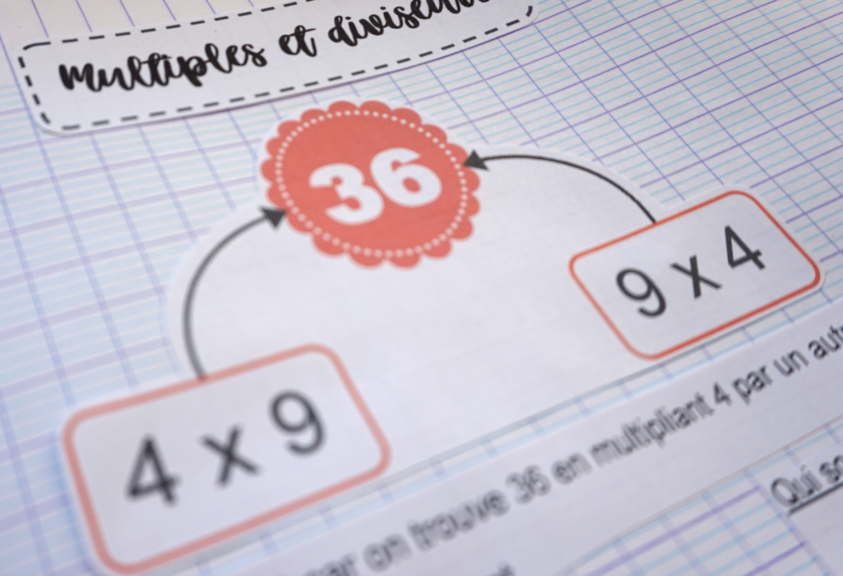
\includegraphics[width=\linewidth]{img/image.png}
		\vspace{-1cm}
	\end{wrapfigure}
	Une variable aléatoire est une fonction qui associe un nombre réel à chaque issue d'une expérience aléatoire.

	$$\Omega \mapsto X(\Omega)$$

	\vspace{3cm}

\end{defi}

\begin{ex}
	On lance un dé équilibré. La variable aléatoire $X$ donne le résultat obtenu.
	\begin{center}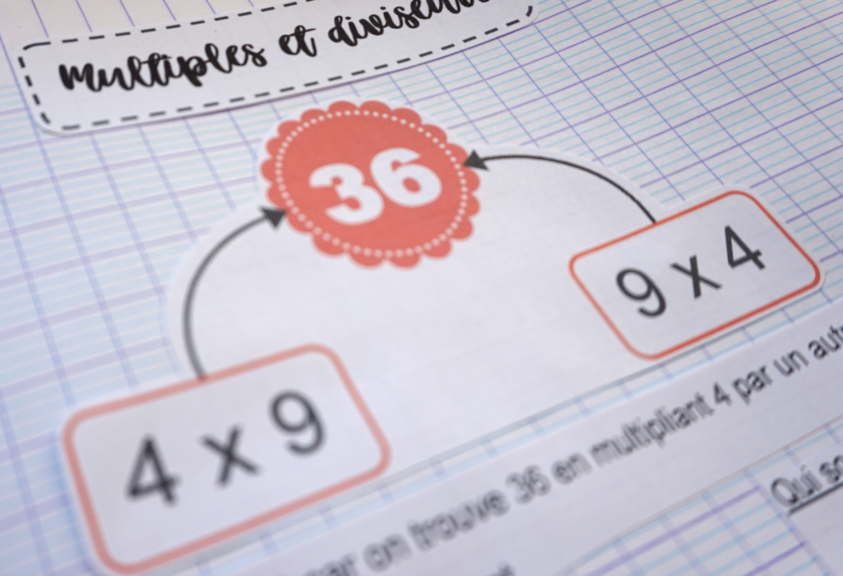
\includegraphics[width=8cm]{img/image.png}\end{center}
\end{ex}

\begin{prop}
	\begin{wrapfigure}{r}{80mm}
		\vspace{-5mm}
		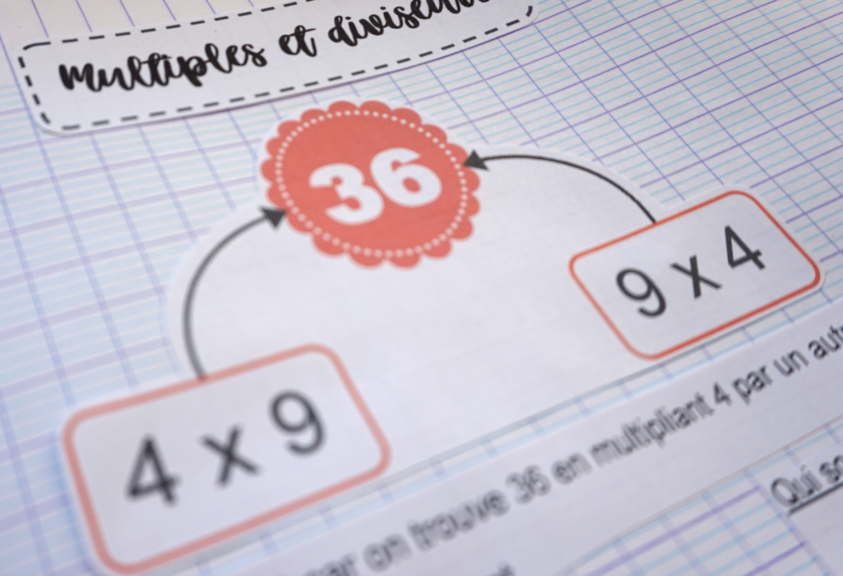
\includegraphics[width=\linewidth]{img/image.png}
		\vspace{-5mm}
	\end{wrapfigure}

	Si $X$ est une variable aléatoire discrète, alors :

	$$\boxed{\sum\limits_{i=0}^{n} \prob(X = x_i) = 1}$$

	\lipsum[3-4]
\end{prop}

\begin{void}
	On peut aussi calculer les prix des pâtes.
	\begin{itemize}
		\item Plop
		      \begin{itemize}
			      \item Plop
			      \item patate
		      \end{itemize}
		\item patate
	\end{itemize}
\end{void}

\subsection{patate}
\subsubsection{ploooooo}

\begin{theo}[Loi des grands nombres]
	Lorsque le \ul{nombre d'expériences} augmente, la moyenne empirique converge vers l'espérance.
\end{theo}

\section{Espérance}

\begin{defi}[Espérance mathématique]
	L'espérance d'une variable aléatoire discrète est définie par :
	$$\esp(X) = \sum_i x_i \prob(X = x_i)$$
\end{defi}

\begin{rem}
	Pour un dé équilibré :
	$\esp(X) = \dfrac{1+2+3+4+5+6}{6} = 3.5$
\end{rem}

\section{Variance}

\begin{defi}
	La variance d'une variable aléatoire est :
	$$\var(X) = \esp\big((X - \esp(X))^2\big)$$
\end{defi}

\begin{prop}
	On a aussi :
	$$\var(X) = \esp(X^2) - \esp(X)^2$$
\end{prop}

\end{document}
